% Written by make_deck_figures.py: edit the script, not this file.
% Equal weights of a 13-ticker basket, scaled by a made-up c = 0.85, with the rest in cash.
\documentclass[tikz,border=2pt]{standalone}
% Shared style for the L15a schematics, copied from L14a (November 19, 2026), \input by each Fig-L15a-*.tex.
% Copied from week-13/L13a/figs/jumphmm-diagram.tex (the week-12 schematic style): same fonts,
% ink, accent colors, boxes, and arrows, plus a monospace font for tool names and order
% statuses. The notebook SVG carries a dark palette added by theme_svg.py; every color here
% must be mapped there.
\usepackage[no-math]{fontspec}
\IfFontExistsTF{Arial}{\setsansfont{Arial}}{\setsansfont{TeX Gyre Heros}}
\renewcommand{\familydefault}{\sfdefault}
\IfFontExistsTF{Menlo}{\setmonofont[Scale=0.92]{Menlo}}{}
\usepackage{amsmath,amssymb}
\usetikzlibrary{arrows.meta,calc,positioning,decorations.pathreplacing}

\definecolor{vnink}{HTML}{202124}
\definecolor{gdblue}{HTML}{0091FF}
\definecolor{gdred}{HTML}{E02020}
\definecolor{gdgray}{HTML}{6D7278}
\definecolor{saorange}{HTML}{F08C00}
\definecolor{boxfill}{HTML}{F1F3F4}
\definecolor{orangefill}{HTML}{FFE8C7}
\definecolor{bluefill}{HTML}{E5F3FF}
\definecolor{redfill}{HTML}{FDE8E8}
\definecolor{gridgray}{HTML}{E3E5E8}

\tikzset{
  every picture/.append style={x=1cm, y=1cm, font=\sffamily\small, text=vnink},
  % boxes and arrows, as in the L12a schematics
  flow/.style={draw=vnink, line width=0.9pt, -{Latex[length=2.4mm, width=1.7mm]}},
  feedback/.style={draw=saorange, line width=1.2pt, -{Latex[length=2.6mm, width=1.9mm]}, rounded corners=6pt},
  sumbox/.style={draw=vnink, fill=boxfill, line width=0.8pt, rounded corners=3pt, inner sep=5pt, align=center},
  note/.style={text=gdgray, font=\sffamily\footnotesize, align=center},
  state/.style={circle, draw=vnink, fill=white, line width=1.0pt, minimum size=1.1cm, inner sep=0pt, font=\sffamily\normalsize},
  % plots, as in the L10b profit diagrams
  axis/.style={draw=vnink, line width=0.8pt, -{Latex[length=2.6mm, width=1.8mm]}},
  spine/.style={draw=vnink, line width=0.8pt},
  curve/.style={draw=vnink, line width=1.6pt, line join=round, line cap=round},
  series/.style={draw=gdgray, line width=0.9pt, line join=round},
  drop/.style={draw=gdgray, line width=0.8pt, dash pattern=on 3pt off 2pt},
  pt/.style={circle, draw=vnink, fill=white, line width=1.0pt, inner sep=0pt, minimum size=2.0mm},
}


\begin{document}
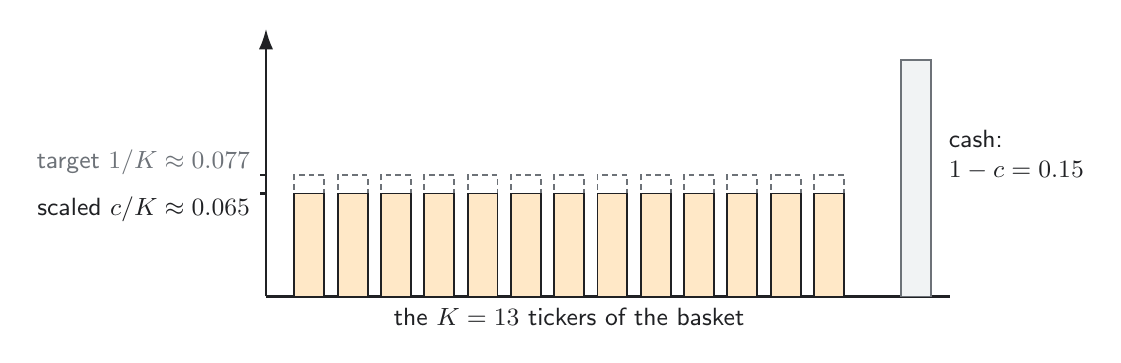
\begin{tikzpicture}
  \draw[axis] (0, 0) -- (0, 3.4);
  \draw[spine] (0, 0) -- (8.69, 0);
  \draw[draw=gdgray, line width=0.7pt, dash pattern=on 2pt off 1.5pt] (0.36, 0) rectangle (0.74, 1.5385);
  \filldraw[fill=orangefill, draw=vnink, line width=0.7pt] (0.36, 0) rectangle (0.74, 1.3077);
  \draw[draw=gdgray, line width=0.7pt, dash pattern=on 2pt off 1.5pt] (0.91, 0) rectangle (1.29, 1.5385);
  \filldraw[fill=orangefill, draw=vnink, line width=0.7pt] (0.91, 0) rectangle (1.29, 1.3077);
  \draw[draw=gdgray, line width=0.7pt, dash pattern=on 2pt off 1.5pt] (1.46, 0) rectangle (1.84, 1.5385);
  \filldraw[fill=orangefill, draw=vnink, line width=0.7pt] (1.46, 0) rectangle (1.84, 1.3077);
  \draw[draw=gdgray, line width=0.7pt, dash pattern=on 2pt off 1.5pt] (2.01, 0) rectangle (2.39, 1.5385);
  \filldraw[fill=orangefill, draw=vnink, line width=0.7pt] (2.01, 0) rectangle (2.39, 1.3077);
  \draw[draw=gdgray, line width=0.7pt, dash pattern=on 2pt off 1.5pt] (2.56, 0) rectangle (2.94, 1.5385);
  \filldraw[fill=orangefill, draw=vnink, line width=0.7pt] (2.56, 0) rectangle (2.94, 1.3077);
  \draw[draw=gdgray, line width=0.7pt, dash pattern=on 2pt off 1.5pt] (3.11, 0) rectangle (3.49, 1.5385);
  \filldraw[fill=orangefill, draw=vnink, line width=0.7pt] (3.11, 0) rectangle (3.49, 1.3077);
  \draw[draw=gdgray, line width=0.7pt, dash pattern=on 2pt off 1.5pt] (3.66, 0) rectangle (4.04, 1.5385);
  \filldraw[fill=orangefill, draw=vnink, line width=0.7pt] (3.66, 0) rectangle (4.04, 1.3077);
  \draw[draw=gdgray, line width=0.7pt, dash pattern=on 2pt off 1.5pt] (4.21, 0) rectangle (4.59, 1.5385);
  \filldraw[fill=orangefill, draw=vnink, line width=0.7pt] (4.21, 0) rectangle (4.59, 1.3077);
  \draw[draw=gdgray, line width=0.7pt, dash pattern=on 2pt off 1.5pt] (4.76, 0) rectangle (5.14, 1.5385);
  \filldraw[fill=orangefill, draw=vnink, line width=0.7pt] (4.76, 0) rectangle (5.14, 1.3077);
  \draw[draw=gdgray, line width=0.7pt, dash pattern=on 2pt off 1.5pt] (5.31, 0) rectangle (5.69, 1.5385);
  \filldraw[fill=orangefill, draw=vnink, line width=0.7pt] (5.31, 0) rectangle (5.69, 1.3077);
  \draw[draw=gdgray, line width=0.7pt, dash pattern=on 2pt off 1.5pt] (5.86, 0) rectangle (6.24, 1.5385);
  \filldraw[fill=orangefill, draw=vnink, line width=0.7pt] (5.86, 0) rectangle (6.24, 1.3077);
  \draw[draw=gdgray, line width=0.7pt, dash pattern=on 2pt off 1.5pt] (6.41, 0) rectangle (6.79, 1.5385);
  \filldraw[fill=orangefill, draw=vnink, line width=0.7pt] (6.41, 0) rectangle (6.79, 1.3077);
  \draw[draw=gdgray, line width=0.7pt, dash pattern=on 2pt off 1.5pt] (6.96, 0) rectangle (7.34, 1.5385);
  \filldraw[fill=orangefill, draw=vnink, line width=0.7pt] (6.96, 0) rectangle (7.34, 1.3077);
  \filldraw[fill=boxfill, draw=gdgray, line width=0.7pt] (8.06, 0) rectangle (8.44, 3);
  \node[font=\sffamily\small, anchor=west, align=left] at (8.55, 1.8) {cash:\\$1-c=0.15$};
  \node[font=\sffamily\small, anchor=north] at (3.85, -0.03) {the $K=13$ tickers of the basket};
  \draw[spine] (0, 1.5385) -- (-0.07, 1.5385);
  \node[anchor=east, font=\sffamily\small, text=gdgray] at (-0.08, 1.6985) {target $1/K\approx 0.077$};
  \draw[spine] (0, 1.3077) -- (-0.07, 1.3077);
  \node[anchor=east, font=\sffamily\small] at (-0.08, 1.1077) {scaled $c/K\approx 0.065$};
\end{tikzpicture}
\end{document}
